\section{Integrazione Simulink dei modelli originali}
\label{sec:simulink-integration}
La verifica implementativa successiva alla PR 32 parte dal commit
\texttt{889c0eb} e dai tre modelli originali di Valerio. Gli archivi sono
conservati senza modifiche in \path{simulink/legacy/valerio}, con hash SHA256
e inventario dei blocchi. Le copie correnti sono in \path{simulink/models}:
\texttt{SEA\_LQG\_integrated}, \texttt{SEA\_LQRI\_integrated},
\texttt{SEA\_Hinf\_integrated} e \texttt{SEA\_Kmu\_integrated}.
Scope, struttura principale, selettori e osservatore sono mantenuti.
Le modifiche correggono le connessioni fisiche e aggiornano i controllori;
non sono state ripetute sintesi, analisi robuste, Monte Carlo o RAS.

\subsection{Correzioni fisiche e coordinate}
Il modello mantiene due sistemi dinamici distinti: la funzione meccanica
restituisce otto derivate e il sottosistema attuatori contiene sei stati.
Il vettore completo incrementale è
\[
 x=\begin{bmatrix}x_{\mathrm{mech}}-\bar x\\x_a-\bar x_a\end{bmatrix},
 \quad x_{\mathrm{mech}}=[q;\dot q;\theta;\dot\theta],\quad
 \bar x_a=-A_a^{-1}B_a\bar\tau.
\]
I parametri provengono da M3. L'ingresso assoluto degli attuatori è
$u_{\mathrm{abs}}=\bar\tau+\delta u+\eta_u$; la loro uscita $\tau$ è la
coppia motore. Il bias di equilibrio compare una sola volta.
La meccanica parte da $\bar x$, mentre controllore e osservatore usano
coordinate incrementali. Un gradino di cinque gradi resta
$r_1=5\pi/180$, anche se il primo link all'equilibrio è a novanta gradi.

Nel modello originale il disturbo era sommato alla coppia motore.
La correzione usa invece
\[
 M(q)\ddot q=K_s(\theta-q)-C(q,\dot q)\dot q-G(q)+d_{\rm ext}+w_d,
\]
lasciando invariata l'equazione del rotore. Il rumore di processo
$w=[w_d;\eta_u]\in\mathbb R^4$ entra nei due canali fisici distinti.
Infatti M3 costruisce $B=[B_mD_a;B_a]$: $\eta_u$ va prima degli attuatori.
Non viene sommato alcun vettore $G_ww\in\mathbb R^{14}$ alla derivata
meccanica di dimensione otto.
La linearizzazione dei diagrammi verifica direttamente la mappa
$G_w=[B_d\ B]$, con errore massimo circa $7.11\,10^{-15}$.

\subsection{Misure, Kalman, azione integrale e 2-DoF}
Il selettore originale $[1,2,5,6]$ è corretto. Alle quattro misure
incrementali si sommano quattro componenti gaussiane indipendenti:
$y_{\rm mis}=y_{\rm ideal}+v$. Gli artifact M6 forniscono
$Q_n=0.01 I_4$ e $R_n=(0.05\pi/180)^2I_4$.
I blocchi Random Number usano un periodo di 0.002 s e seed distinti;
la loro varianza è quella dichiarata. Questa è una convenzione numerica
ZOH a banda finita, non un'identificazione esatta con le intensità del
rumore bianco continuo utilizzate da \texttt{lqe}.
Tre interruttori indipendenti attivano disturbo deterministico, rumore di
processo e rumore di misura.

L'osservatore originale è mantenuto e realizza
$\dot{\hat x}=A\hat x+B\delta u+L(y_{\rm mis}-C\hat x)$.
Il controllo LQG usa $-K\hat x+N_rr$; LQRI usa
$-K_x\hat x-K_i\xi$, con $\dot\xi=r-[I_2\ 0]y_{\rm mis}$.
È stato corretto il collegamento originale che integrava la misura ideale.
Non è presente un prefiltro nel diagramma LQRI.
I due modelli robusti ricevono $[r;q_{\rm mis}]$ con quattro ingressi;
ciascuno mantiene l'intera realizzazione salvata, con stati condivisi fra
ramo di riferimento e ramo di misura. Nessun osservatore aggiuntivo,
\texttt{minreal}, riduzione d'ordine o vecchio command shaping è introdotto.
Le chiusure hanno rispettivamente 28, 30, 36 e 92 stati continui.

\subsection{Verifiche numeriche e significato del PASS}
La suite dedicata ha superato 67 controlli e sette test
\texttt{matlab.unittest} su MATLAB/Simulink R2025b.
Il solver è \texttt{ode23t}, con tolleranze $10^{-7}$ e $10^{-9}$ e passo
massimo 0.002 s. I segnali \texttt{logsout} vengono ricampionati sulla
griglia di 0.002 s; gli artifact conservano queste traiettorie, evitando
copie ridondanti delle registrazioni adattive.

Il confronto indipendente chiude il controllore salvato sulla pianta M3 e
usa \texttt{lsim}. L'eccitazione simultanea è $[10^{-4};-7\,10^{-5}]$ rad,
con orizzonte tre secondi, rumori e disturbo disattivati.
Le tolleranze prefissate sono $2\,10^{-7}$ rad per $q$ e $2\,10^{-4}$ N m
per $u$. Il primo limite equivale allo 0.2\% dell'eccitazione principale;
il secondo ammette l'errore di interpolazione dei transitori stiff.
Il confronto attuatori usa la realizzazione M3 e il medesimo ingresso
registrato, entro $2\,10^{-4}$ N m.
\begin{table}[htbp]\centering\small
\begin{tabular}{lrrrr}\toprule
Controllore & max errore $q$ & RMS errore $q$ & max errore $u$ & errore $G_w$\\\midrule
LQG & 7.63e-10 & 8.31e-11 & 1.55e-07 & 7.11e-15 \\
LQRI & 2.96e-10 & 4.11e-11 & 3.82e-08 & 7.11e-15 \\
Hinf & 8.88e-10 & 2.65e-10 & 4.87e-08 & 7.11e-15 \\
Kmu & 1.03e-09 & 3.23e-10 & 1.21e-08 & 7.11e-15 \\
\bottomrule\end{tabular}
\caption{Equivalenza locale: posizioni in rad, comandi in N m.}
\end{table}
\begin{figure}[htbp]\centering
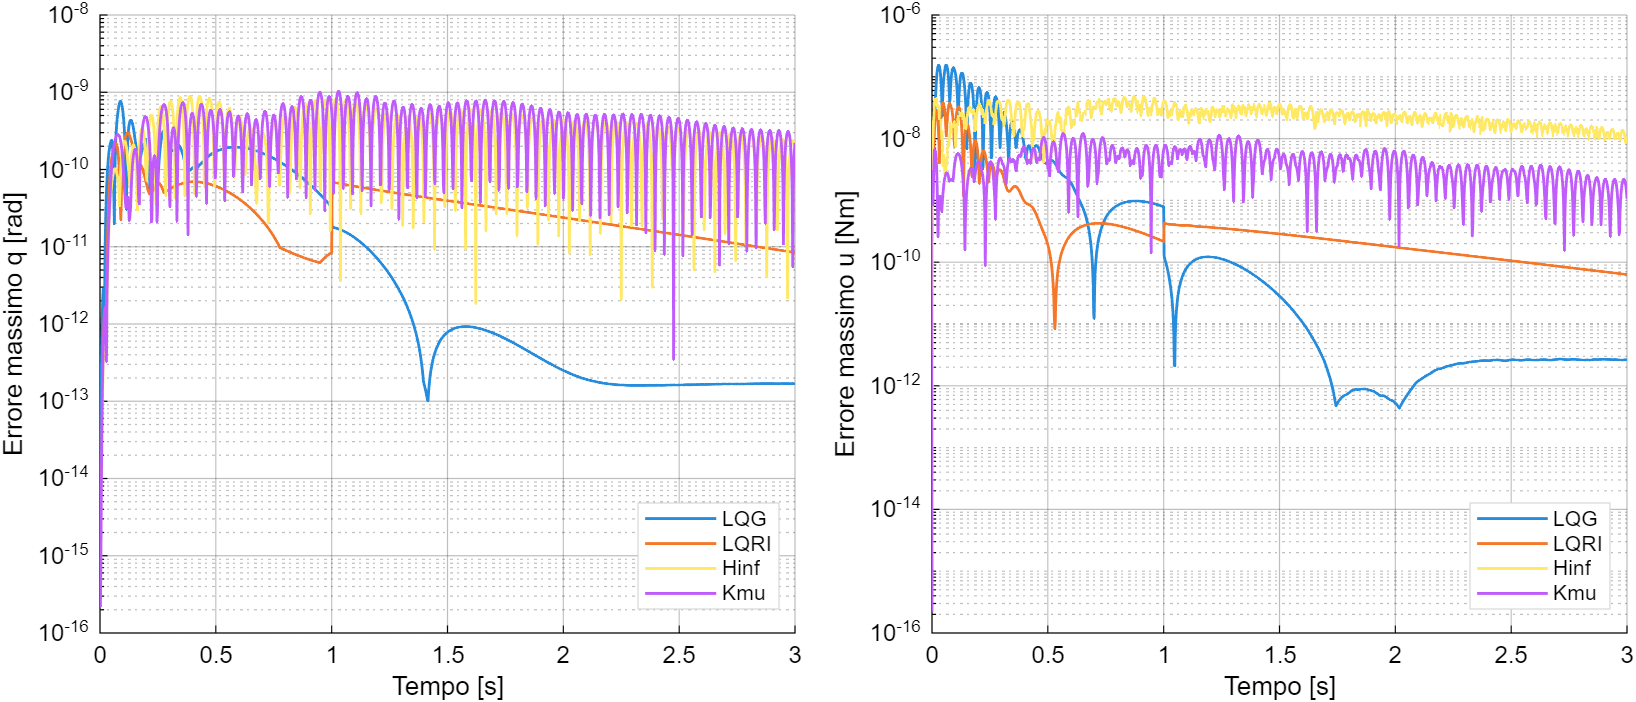
\includegraphics[width=\textwidth]{figures/simulink_integration/equivalence.png}
\caption{Errori fra i diagrammi non lineari Simulink e le mappe lineari MATLAB.}
\end{figure}

Con un errore iniziale di stima $10^{-4}$ sul primo stato, in assenza di
rumore, il residuo dello stimatore a tre secondi è inferiore a
$1.3\,10^{-14}$ per LQG e LQRI. Nella breve prova con entrambi i rumori
l'RMS aggregato degli errori di stima è circa 0.01062; poiché include
coordinate fisiche e stati interni dell'attuatore con scale diverse,
non va interpretato come un errore angolare RMS.
Tutte le ripetizioni con gli stessi seed producono differenza nulla sul
comando. Le prove di rumore durano soltanto 0.5 s: verificano collegamenti,
finitezza e ripetibilità, non sostituiscono la campagna M15 di quattro secondi.
In particolare non annullano il grave limite H-infinity già documentato.

\subsection{Tracking e dimostrazione dell'integratore}
La tabella riporta due gradini separati di cinque gradi e quattro secondi.
L'errore finale è stimato sugli ultimi 0.2 s; l'assestamento usa una fascia
del 2\% dell'ampiezza del riferimento attorno a tale valore.
Si conservano overshoot rispetto al riferimento, rapporto di cross coupling,
picco assoluto e RMS dei due comandi su tutto l'orizzonte.
Per LQRI il valore di coda a quattro secondi non coincide con il limite
asintotico: non viene presentato come errore statico certificato.
\begin{table}[htbp]\centering\small
\begin{tabular}{lrrrrrr}\toprule
Caso/giunto & $T_s$ [s] & OS [\%] & $e_f/r$ & cross & picco $u$ & RMS $u$\\\midrule
LQG / 1 & 0.668 & 0.283 & 0.00155 & 0.1693 & 4.746 & 0.6195 \\
LQG / 2 & 0.474 & 0 & 0.000752 & 0.169 & 4.511 & 0.2383 \\
LQRI / 1 & 3.504 & 0 & 0.05193 & 0.0377 & 0.784 & 0.4296 \\
LQRI / 2 & 3.424 & 0 & 0.03931 & 0.03729 & 0.1975 & 0.1487 \\
Hinf / 1 & 1.46 & 0 & 0.005181 & 0.01425 & 0.8683 & 0.5621 \\
Hinf / 2 & 1.46 & 0 & 0.002475 & 0.01055 & 0.2439 & 0.1922 \\
Kmu / 1 & 1.524 & 0 & 0.0602 & 0.1043 & 0.7964 & 0.4993 \\
Kmu / 2 & 1.484 & 0 & 0.03075 & 0.1099 & 0.1992 & 0.1728 \\
\bottomrule\end{tabular}
\caption{Metriche delle nuove simulazioni; comandi in N m. I target M5 rimangono invariati.}
\end{table}
\begin{figure}[p]\centering
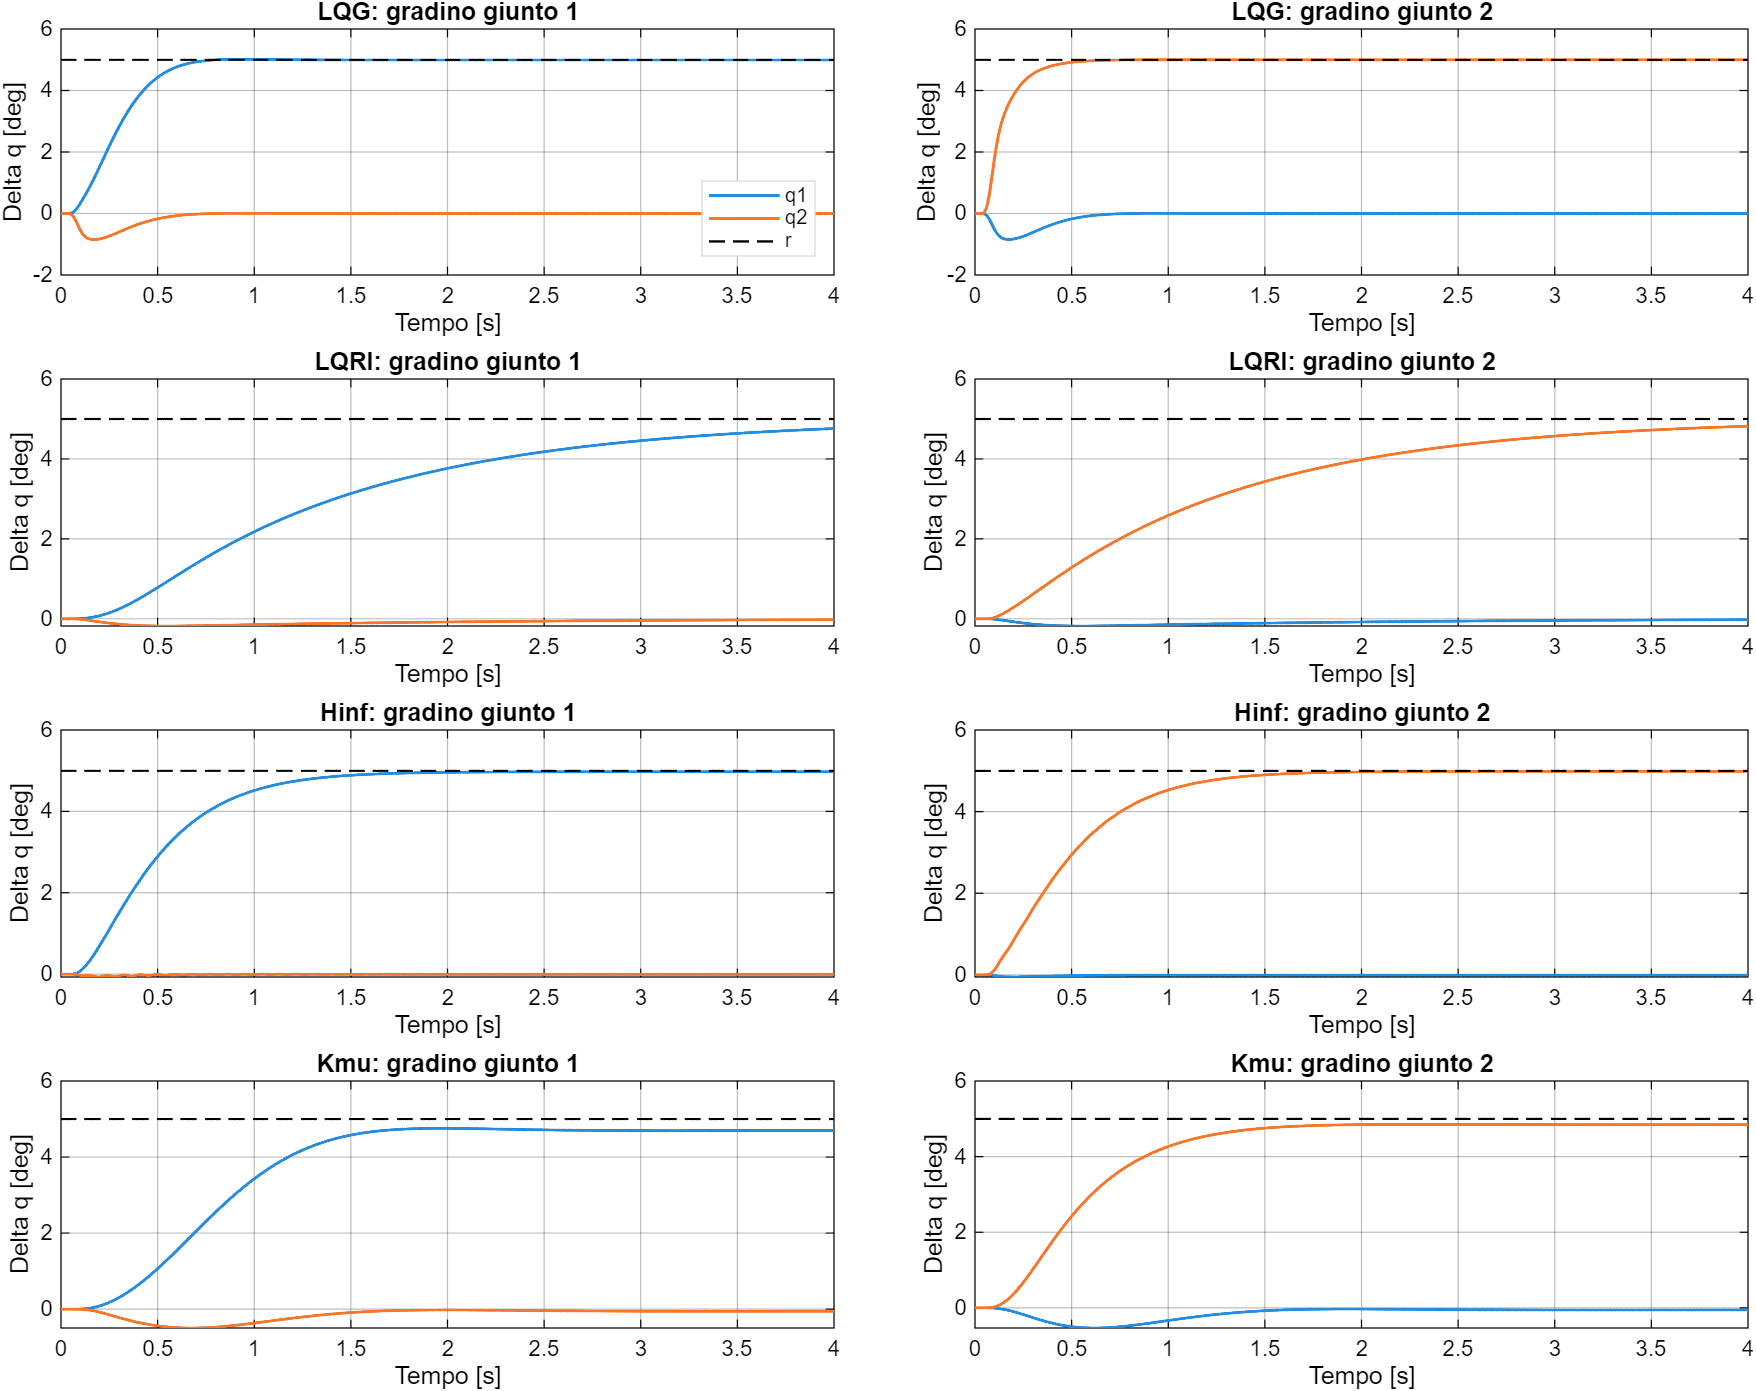
\includegraphics[width=.98\textwidth]{figures/simulink_integration/tracking.png}
\caption{Tracking nei quattro modelli integrati, con identica pianta fisica.}
\end{figure}

A riferimento nullo si applica $d_{\rm ext}=[0.5;0]$ N m da $t=1$ s,
con rumori disattivati e orizzonte 20 s. LQG converge a circa
$[0.07183;-0.02802]$ rad; LQRI lascia circa
$[1.775\,10^{-8};1.082\,10^{-9}]$ rad nella media finale di 0.5 s.
Il rapporto delle norme è $2.306\,10^{-7}$.
Questo confronto dimostra la reiezione del disturbo costante per il caso
simulato, senza attribuire a M7 conformità M5 o garanzie robuste ulteriori.
\begin{figure}[htbp]\centering
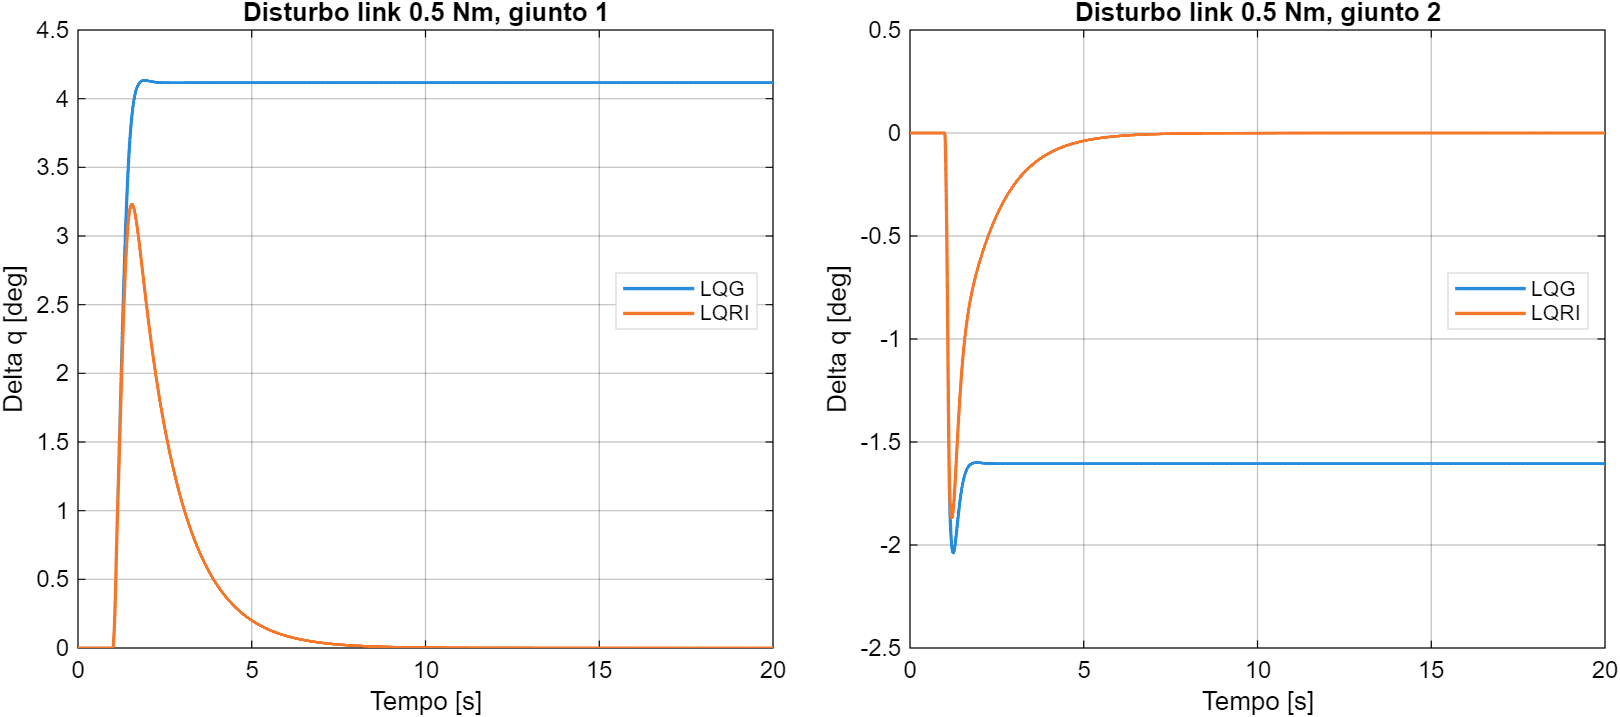
\includegraphics[width=\textwidth]{figures/simulink_integration/disturbance.png}
\caption{Stesso disturbo sul primo link: offset LQG e recupero LQRI.}
\end{figure}

\subsection{Riproducibilità e limiti di compatibilità}
Il comando \texttt{setenv('CR\_RUN\_SCOPE','simulink'); run\_all}
riesegue esclusivamente questa verifica. I quattro script
\path{simulink/setup_*_simulink.m} aprono i modelli con parametri caricati dagli
artifact; \path{build_simulink_integration.m} ricostruisce le copie dagli originali.
Questi ultimi sono R2026a: l'importazione su R2025b segnala metadati non
riconosciuti e il riferimento \texttt{cstblocks\_lti} non risolto.
Nelle copie, il sottosistema attuatori utilizza blocchi State-Space standard
con le matrici M3; il bus di parametri esterno \texttt{slBus1} è sostituito da
un vettore di 17 parametri, ricomposto in struttura dentro la funzione.
Quel vettore contiene parametri, non stati aggiuntivi.
Gli originali restano intatti e la preferenza di importazione viene ripristinata.
I modelli corretti sono effettivamente compilati e simulati: non sono solo
script predisposti per una futura esecuzione. Non è stata verificata
separatamente la loro esecuzione su R2026a, né la generazione di codice o
l'hardware. Il PASS implementativo non modifica H-infinity RS FAIL,
Monte Carlo 0/40, Kmu RS/RP PASS e 40/40, M5 FAIL per entrambi e M7 PARTIAL.
